\documentclass[12pt,a4paper,twoside]{article}
% Adapted from ReportTemplate/template.tex.
\newcommand{\studentname}{Xie Boyang}
\newcommand{\studentnumber}{24020036030}
\newcommand{\labgroup}{6}
\title{Lab 3 Report\\[0.3em]\large Quadrotor modelling and geometric trajectory control}
\usepackage[a4paper,left=25mm,right=25mm,bottom=25mm,top=25mm]{geometry}
\usepackage[T1]{fontenc}
\usepackage{lmodern}
\usepackage[british]{babel}
\usepackage{amsmath,amssymb,graphicx,booktabs,array,fancyhdr}
\usepackage[square,comma,numbers,sort&compress]{natbib}
\usepackage{microtype}
\usepackage{listings}
\usepackage{caption}
\usepackage{float}
\usepackage[hidelinks]{hyperref}
\captionsetup{font=small,labelfont=bf}
\lstset{language=C++,basicstyle=\ttfamily\small,breaklines=true,columns=fullflexible,keepspaces=true,showstringspaces=false,frame=single,framerule=.3pt,xleftmargin=3pt,xrightmargin=3pt}
\setlength{\parindent}{0pt}
\setlength{\parskip}{0.45em}
\setlength{\headheight}{15pt}
\setlength{\emergencystretch}{2em}
\pagestyle{fancy}
\fancyhf{}
\fancyhead[C]{\small Lab 3: Quadrotor geometric control}
\fancyfoot[C]{\thepage}
\renewcommand{\headrulewidth}{0pt}
\renewcommand{\footrulewidth}{0pt}
\renewcommand{\abstractname}{Summary}
\author{\small Name: \studentname\\[0.4em]\small Student number: \studentnumber\\[0.4em]\small Lab group: \labgroup\\[0.4em]\small Code: \url{https://github.com/chixin114514/2026Fall_TeamFullcans/tree/main/lab3}}
\date{}
\hypersetup{pdftitle={Lab 3 Report: Quadrotor modelling and geometric trajectory control}}
\raggedbottom
% Let figures share pages with text and stack float pages from the top.
\renewcommand{\topfraction}{0.9}
\renewcommand{\bottomfraction}{0.8}
\renewcommand{\textfraction}{0.07}
\renewcommand{\floatpagefraction}{0.8}
\setcounter{topnumber}{3}
\setcounter{totalnumber}{4}
\makeatletter
\setlength{\@fptop}{0pt}
\setlength{\@fpsep}{12pt plus 2fil}
\setlength{\@fpbot}{0pt plus 1fil}
\makeatother
\begin{document}
\renewcommand{\abstractname}{Summary}
\maketitle
\begin{abstract}
A quadrotor tracks a trajectory only if every link from the reference to the motors agrees on rotation, thrust and rotor conventions. This report builds that chain from quaternion conversion to a ROS geometric controller and validates it in the Unity/TESSE simulator provided by MIT. The rotor-allocation analysis proves that reversing two propellers removes independent yaw authority (rank 4 drops to rank 3). A body-frame quadratic drag model yields an explicit compensation term. On the simulator with 50 Hz state feedback, the controller holds the 5 m, 2.5 m\,s$^{-1}$ circle to a radial RMS error of 2.4 mm (0.05\% of the radius) and a three-dimensional RMS error of 4.1 cm. A constant along-track offset of 14.5 ms of reference time accounts for 86\% of the remaining squared error, and the 1.5 cm height offset matches the proportional thrust balance to 1\%. A start sequence takes the vehicle from its spawn pose to the circle without overshoot.
\end{abstract}

\section{Lab Introduction and Team Information}
Quadrotor trajectory tracking requires a consistent connection between state coordinates and motor commands. A correct feedback equation can generate the wrong motion if the rotation direction, thrust sign or rotor numbering changes between the model and the simulator. This lab examines that connection through the individual exercises and the ROS controller implementation specified in MIT VNAV Lab 3~\citep{vnav}.

The report follows the three deliverables: quaternion conversions, modelling and control analysis, and geometric control of a simulated UAV. The control loop adapts the geometric approach of \citet{lee2010} to an upward world and body $z$ axis. The flight is recorded simultaneously in Unity and RViz. The code, configuration and flight logs are available at \url{https://github.com/chixin114514/2026Fall_TeamFullcans/tree/main/lab3}.

The main result is the accuracy of the circle's geometry. After the first two periods, the measured path stays within 5.3 mm of the 5 m radius. Decomposing the error along the reference's moving frame shows where the remaining 4.1 cm comes from: a constant timing offset along the path and a 1.5 cm height offset set by the proportional gain.

\textit{My responsibility: ROS communication and simulation integration.} I set up the ROS Noetic workspace, its dependencies and the container runtime; connected TESSE, the ROS bridge and the controller; checked the state, command and simulation-clock communication; took part in resolving compatibility issues and in joint testing; and wrote the system-implementation part of this report.

\section{Individual Work}
\subsection{Deliverable 1: From attitude messages to control variables}
The controller receives the drone's orientation as a quaternion in a ROS message. Its feedback equations need a rotation matrix, while the desired heading is specified by a yaw angle. This exercise explains how to obtain those quantities from the received data.

Three C++ types appear in this process. A \texttt{geometry\_msgs::Quaternion} carries the four components $(x,y,z,w)$ between ROS nodes. A \texttt{tf2::Quaternion} stores the same rotation in a form supported by the tf2 rotation utilities. An \texttt{Eigen::Matrix3d} stores the corresponding $3\times3$ rotation matrix for matrix and vector calculations. Converting between the quaternion and matrix representations preserves the represented orientation; extracting yaw selects its heading component.

\subsubsection*{A. Reading and writing quaternion data (A1--A3)}
For A1, suppose \texttt{quat\_msg} is the received message and \texttt{quat\_tf} is an already declared tf2 quaternion. The following call copies the message components into \texttt{quat\_tf}~\citep{rosgeometry}:
\begin{lstlisting}
tf2::fromMsg(quat_msg, quat_tf);
\end{lstlisting}
For A2, the reverse operation creates a ROS message from a computed tf2 quaternion. This is useful when an orientation must be published to another node:
\begin{lstlisting}
geometry_msgs::Quaternion quat_msg = tf2::toMsg(quat_tf);
\end{lstlisting}
The three snippets are independent; variable names follow the exercise.

For A3, the scalar component of the quaternion is obtained with:
\begin{lstlisting}
quat_tf.w();
\end{lstlisting}
A quaternion contains a vector part $(x,y,z)$ and a scalar part $w$. Reading $w$ returns one stored component. Calculating yaw requires the rotation represented by the quaternion, as shown next.

\subsubsection*{B. Obtaining heading and a rotation matrix (B1--B2)}
For B1, extract yaw from the tf2 quaternion \texttt{quat\_t} with one function call~\citep{rosutils}:
\begin{lstlisting}
double yaw = tf2::getYaw(quat_t);
\end{lstlisting}
The result is a heading angle in radians. In this lab, the desired-state callback uses this operation to obtain $\psi_d$ from the reference orientation. The controller then uses $\psi_d$ to construct its desired heading direction.

For B2, convert a ROS quaternion message into an Eigen quaternion, then convert that quaternion into a rotation matrix~\citep{roseigen}:
\begin{lstlisting}
Eigen::Quaterniond q_eigen;
tf2::fromMsg(quat_msg, q_eigen);
Eigen::Matrix3d R = q_eigen.toRotationMatrix();
\end{lstlisting}
The first line declares storage; the next two lines perform the two requested conversions. The input is treated as a unit quaternion; the current-state callback checks and normalises it before forming $R$.

For the current attitude in this lab, $R$ maps a body-frame vector to the world frame: $v^w=Rv^b$. Its transpose performs the reverse conversion. The controller therefore computes $\Omega=R^T\Omega_{\mathrm{world}}$ to express the received angular velocity in body coordinates. It also uses $R$ to calculate attitude error and the current thrust direction. Thus yaw extraction supplies the desired heading, while matrix conversion supplies the current attitude needed by the feedback equations.

\subsection{Deliverable 2A: Rotor layout and control authority}
Use the top view in Figure~\ref{fig:rotors}, with $x$ to the right, $y$ upward on the page and $z$ out of the page. Let $d$ be the centre-to-rotor distance, $a=d/\sqrt{2}$, $c_f>0$ the lift coefficient and $c_d>0$ the yaw reaction-torque coefficient. The individual exercise numbers the rotor positions as
\begin{equation}
 \rho_1=(-a,a,0)^T,\quad \rho_2=(-a,-a,0)^T,\quad
 \rho_3=(a,-a,0)^T,\quad \rho_4=(a,a,0)^T.
\end{equation}

\begin{figure}[!htbp]
\centering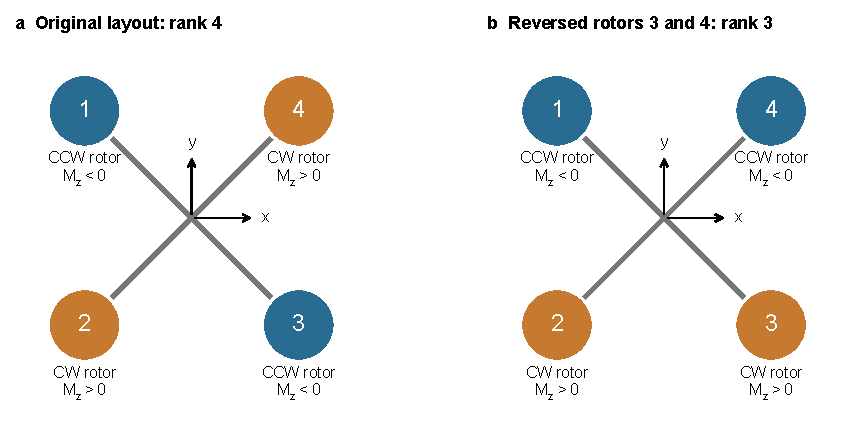
\includegraphics[width=\linewidth]{figures/rotor_layout.pdf}
\caption{Rotor configurations for the individual exercise. CW and CCW denote rotation viewed from above; the indicated $M_z$ is the resulting body reaction torque. Reversing rotors 3 and 4, with matching propeller types, preserves upward lift and changes the yaw-torque signs. Diagram redrawn from the course configuration~\citep{vnav}.}
\label{fig:rotors}
\end{figure}

Let $u_i=\omega_i^2\geq0$, with $\omega_i$ measured in each rotor's configured lifting direction. The force is $f_i=c_fu_i$, and the moment arm gives
\begin{equation}
 \rho_i\times(0,0,f_i)^T=(\rho_{iy}f_i,-\rho_{ix}f_i,0)^T.
\end{equation}
For the wrench $w=(f,M_x,M_y,M_z)^T$, configuration (a) therefore has
\begin{equation}
 w=F_a u,\qquad
 F_a=\begin{bmatrix}
 c_f&c_f&c_f&c_f\\
 ac_f&-ac_f&-ac_f&ac_f\\
 ac_f&ac_f&-ac_f&-ac_f\\
 -c_d&c_d&-c_d&c_d
 \end{bmatrix}.
 \label{eq:fa}
\end{equation}
After division by their nonzero scale factors, the four rows are mutually orthogonal. Consequently,
\begin{equation}
 \det F_a=16a^2c_f^3c_d=8d^2c_f^3c_d\ne0,
 \qquad \operatorname{rank}(F_a)=4.
\end{equation}
All four wrench components can be adjusted independently near a positive-speed hover, within actuator limits.

For configuration (b), only the last row changes:
\begin{equation}
 F_b=\begin{bmatrix}
 c_f&c_f&c_f&c_f\\
 ac_f&-ac_f&-ac_f&ac_f\\
 ac_f&ac_f&-ac_f&-ac_f\\
 -c_d&c_d&c_d&-c_d
 \end{bmatrix}.
 \label{eq:fb}
\end{equation}
The last row equals $-c_d/(ac_f)$ times the second row. The other three rows remain independent, so
\begin{equation}
 \boxed{\operatorname{rank}(F_b)=3,\qquad M_z=-\frac{c_d}{ac_f}M_x.}
\end{equation}
For example, $F_b(1,-1,1,-1)^T=0$. At level hover with zero angular velocity, holding position while starting a pure yaw rotation requires zero roll moment and a nonzero yaw moment. The constraint above makes that command impossible. Configuration (b) therefore cannot track an arbitrary independently prescribed trajectory $(x,y,z,\Psi)$.

\subsection{Deliverable 2B: Compensation for quadratic body drag}
Let $R\in SO(3)$ map body vectors to world coordinates and let $v$ be world velocity. The drag law in the assignment becomes
\begin{equation}
 v^b=R^Tv,\qquad D=\operatorname{diag}(0.1,0.1,0.2),\qquad
 F_D^b=-D\bigl(v^b\odot|v^b|\bigr),\qquad F_D^w=RF_D^b,
\end{equation}
where $\odot$ denotes componentwise multiplication. Its sign is physically consistent because
\begin{equation}
 (v^b)^TF_D^b=-0.1|v_x^b|^3-0.1|v_y^b|^3-0.2|v_z^b|^3\leq0.
\end{equation}
With $e_3=(0,0,1)^T$ and upward $z$, translation obeys
\begin{equation}
 m\dot v=-mg e_3+fRe_3+F_D^w.
\end{equation}
Define $e_x=x-x_d$ and $e_v=v-v_d$. Subtract the estimated world-frame drag from the commanded force:
\begin{equation}
 \boxed{A=-k_xe_x-k_ve_v+mg e_3+m\ddot x_d-\widehat F_D^w.}
 \label{eq:drag}
\end{equation}
Compute the estimate from measured velocity and attitude, then use this same $A$ for both the desired thrust direction and thrust magnitude. If the attitude follows that direction and the drag estimate is exact, substitution into the dynamics gives $m\dot e_v=-k_xe_x-k_ve_v$. Otherwise, the remaining terms include attitude tracking error and $F_D^w-\widehat F_D^w$.

\begin{figure}[!htbp]
\centering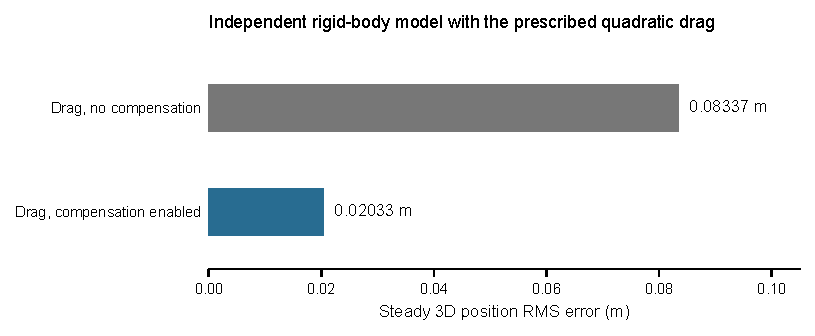
\includegraphics[width=.9\linewidth]{figures/drag_compensation.pdf}
\caption{Recorded compensation comparison in the independent rigid-body model. One deterministic simulation per condition, 1 ms integration step, with the prescribed quadratic drag; RMS error is evaluated after two circular periods. Gains $(k_x,k_v,k_R,k_\Omega)=(6,4.7,64,16)$ from the validation log.}
\label{fig:drag}
\end{figure}

The numerical comparison in Figure~\ref{fig:drag} reduced the recorded RMS error from 0.08337 m to 0.02033 m, a reduction of 75.6\%. This result confirms that the compensation term removes the drag it models. The TESSE flight runs with the compensation disabled (\texttt{compensate\_drag: false}) so that drag already included in the simulator is not modelled twice.

\section{Team Work}
\subsection{Deliverable 3: ROS control architecture}
The controller closes the loop between the trajectory publisher and the unmodified TESSE simulator executable through the ROS bridge (Figure~\ref{fig:loop}). Its three interfaces are \texttt{/desired\_state}, \texttt{/current\_state} and \texttt{/rotor\_speed\_cmds}. They carry \texttt{MultiDOFJointTrajectoryPoint}, \texttt{Odometry} and \texttt{Actuators} messages, respectively.

\begin{figure}[!htbp]
\centering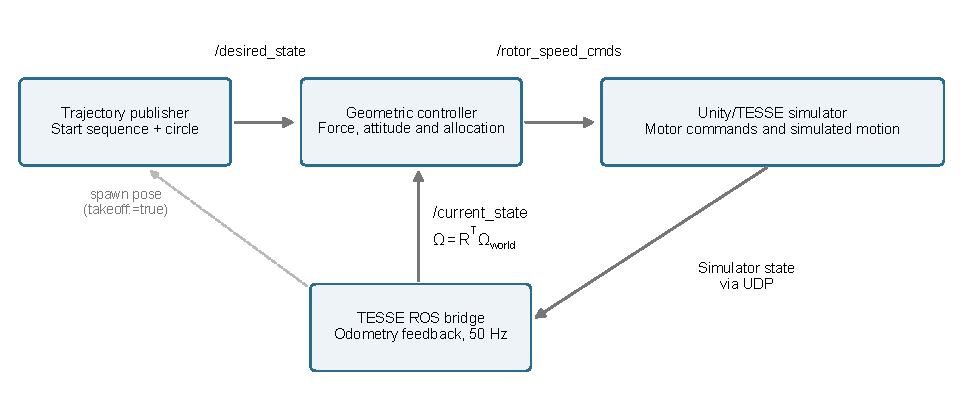
\includegraphics[width=\linewidth]{figures/control_loop.pdf}
\caption{Implemented control loop. The trajectory publisher reads the spawn pose once and then streams position, velocity, acceleration and yaw. The controller converts the received world-frame angular velocity to the body frame, computes thrust and moments, and allocates them to four signed rotor speeds. The bridge returns the simulated state at 50 Hz.}
\label{fig:loop}
\end{figure}

The controller accepts a message only after checking array sizes, finite values and the quaternion norm, then stores the latest valid reference and measurement. It stops publishing commands when either input is more than 1 s old, and its timer runs at 200 Hz.

The simulator renders at several hundred frames per second (Figure~\ref{fig:views}a) and delivers \texttt{/current\_state} at 50 Hz. The controller's model constants are $m=1$ kg, $g=9.81$ m\,s$^{-2}$, $d=0.3$ m, $c_f=10^{-3}$, $c_d=10^{-5}$ and $J=I_3$, with angular speed in rad\,s$^{-1}$.

\subsection{Geometric feedback and rotor allocation}
The commanded force is Equation~\eqref{eq:drag} without the drag term. The reference heading is $b_{1c}=(\cos\psi_d,\sin\psi_d,0)^T$. The desired attitude follows from
\begin{equation}
 b_{3d}=\frac{A}{\|A\|},\qquad
 b_{2d}=\frac{b_{3d}\times b_{1c}}{\|b_{3d}\times b_{1c}\|},\qquad
 R_d=[\,b_{2d}\times b_{3d}\quad b_{2d}\quad b_{3d}\,].
\end{equation}
The positive $b_{3d}$ sign matches the upward thrust convention. A near-zero force falls back to a vertical direction, and a degenerate cross product falls back to a perpendicular heading.

The attitude error, thrust and moment are
\begin{align}
 e_R&=\tfrac12\bigl(R_d^TR-R^TR_d\bigr)^\vee,\\
 f&=A\cdot Re_3,\\
 M&=-k_R e_R-k_\Omega\Omega+\Omega\times(J\Omega).
 \label{eq:moment}
\end{align}
The vee map returns $(S_{32},S_{13},S_{21})^T$ for a skew-symmetric matrix $S$. The attitude law uses $\Omega_d=\dot\Omega_d=0$, as the exercise permits. The measured angular velocity is transformed as $\Omega=R^T\Omega_{\mathrm{world}}$ before Equation~\eqref{eq:moment} is applied.

The simulator numbers its rotors differently from Equation~\eqref{eq:fa}. Its positions are $(a,a,0)$, $(-a,a,0)$, $(-a,-a,0)$ and $(a,-a,0)$ for rotors 1 to 4. With $s_i=\omega_i|\omega_i|$, the implemented map is
\begin{equation}
 \begin{bmatrix}f\\M_x\\M_y\\M_z\end{bmatrix}
 =F_{\mathrm{sim}}s,\qquad
 F_{\mathrm{sim}}=\begin{bmatrix}
 c_f&c_f&c_f&c_f\\
 ac_f&ac_f&-ac_f&-ac_f\\
 -ac_f&ac_f&ac_f&-ac_f\\
 c_d&-c_d&c_d&-c_d
 \end{bmatrix}.
 \label{eq:fsim}
\end{equation}
The inverse is computed once. Each update obtains $s=F_{\mathrm{sim}}^{-1}w$ and publishes $\omega_i=\operatorname{sign}(s_i)\sqrt{|s_i|}$. The signed square root follows the simulator's reversible-rotor input convention.

\subsection{Reference trajectory and start sequence}
The official circular reference is
\begin{align}
 x_d(t)&=(5\sin(t/2),\,5\cos(t/2),\,2)^T, & \psi_d(t)&=-t/2,\\
 v_d(t)&=(2.5\cos(t/2),\,-2.5\sin(t/2),\,0)^T,\\
 a_d(t)&=(-1.25\sin(t/2),\,-1.25\cos(t/2),\,0)^T,
\end{align}
with radius 5 m, speed 2.5 m\,s$^{-1}$ and period $T=4\pi\approx12.566$ s.

The vehicle spawns at $(0,0,0.70)$ m with yaw $-166^\circ$, so starting this reference directly at $t=0$ would demand a 5 m jump and a $166^\circ$ turn while the reference already moves at 2.5 m\,s$^{-1}$. In earlier runs that start drove body rates to about $400^\circ$\,s$^{-1}$ and climbed to 2.6--2.9 m. The trajectory publisher therefore reads the spawn pose and runs three stages at negative trajectory time (\texttt{takeoff:=true}):
\begin{enumerate}
 \item a 6 s straight-line transfer to the circle start $(0,5,2)$ with the minimum-jerk profile $\sigma(u)=10u^3-15u^4+6u^5$, turning yaw the short way to $0^\circ$;
 \item a 3 s hover at the circle start;
 \item a 6 s ramp, centred on $t=0$, in which the phase rate rises smoothly from 0 to $\tfrac12$ rad\,s$^{-1}$.
\end{enumerate}
From $t=3$ s onwards the reference is exactly the official circle above. Position, velocity and acceleration remain continuous across every stage boundary.

\subsection{Evaluation}
The flight log records the state at 50 Hz over trajectory times $-12$ to 55.08 s. At each state callback, the logger pairs the state with the latest received reference. Samples with $t<0$ cover the start sequence. Steady statistics use the established window $t\geq2T=25.13$ s.

For the steady sample set $\mathcal{S}$, the position and radius errors are
\begin{equation}
 E_p=\sqrt{\frac{1}{|\mathcal{S}|}\sum_{i\in\mathcal{S}}\|x_i-x_{d,i}\|^2},\qquad
 E_r=\sqrt{\frac{1}{|\mathcal{S}|}\sum_{i\in\mathcal{S}}
 \left(\sqrt{x_i^2+y_i^2}-5\right)^2}.
\end{equation}
The planar error is also resolved along the reference's unit tangent $\tau=(\cos\tfrac t2,-\sin\tfrac t2)$ and unit radius $\rho=(\sin\tfrac t2,\cos\tfrac t2)$. Together with the vertical axis these form an orthonormal frame, so the three mean squared components sum exactly to $E_p^2$. Turns are counted from the unwrapped measured phase $\operatorname{atan2}(x_i,y_i)$.

\subsection{Tracking result}
Figure~\ref{fig:tracking} shows the complete flight. The measured path lies on the reference circle throughout: in the steady window the radius error has an RMS of 2.4 mm and never exceeds 5.3 mm. A least-squares circle fitted to the measured path has radius 4.9978 m and a centre within 0.1 mm of the origin. The vehicle completes 2.38 measured turns in the window, and the height stays between 1.981 and 1.988 m.

\begin{figure}[!htbp]
\centering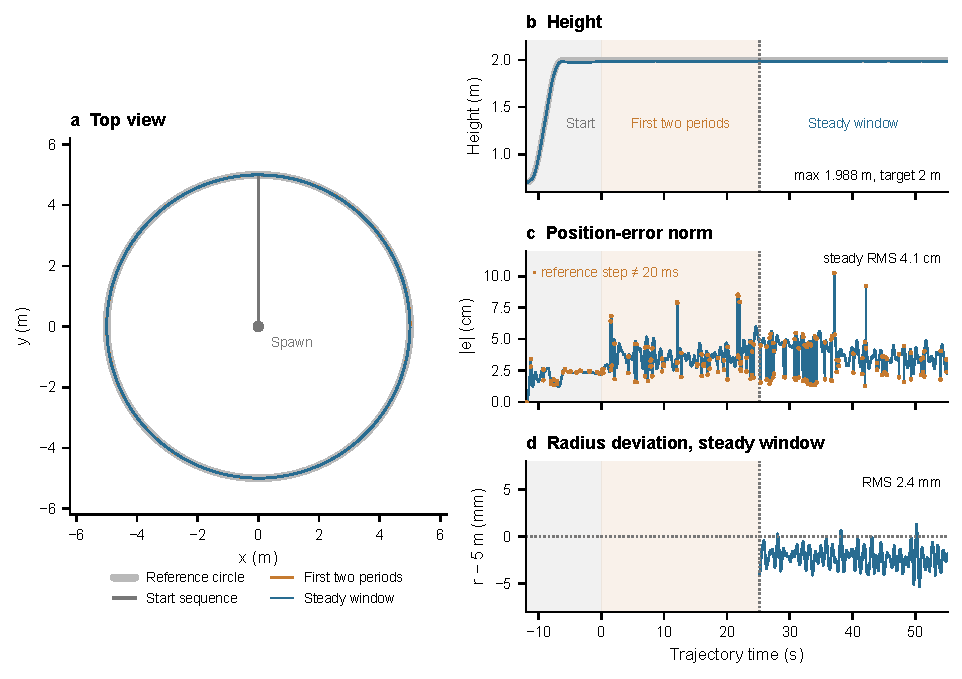
\includegraphics[width=\linewidth]{figures/official_tracking.pdf}
\caption{TESSE flight. (a) Top view: start sequence (grey), first two periods (orange) and steady window (blue) over the wide reference circle. (b) Measured height against the 2 m target. (c) Three-dimensional position-error norm. Orange dots mark samples whose paired reference advanced by 0 or 40 ms instead of 20 ms. (d) Deviation of the measured radius from 5 m in the steady window. Shading in (b--d) marks the start sequence and the first two periods; the dotted line marks $t=8\pi$ s.}
\label{fig:tracking}
\end{figure}



The error decomposition in Figure~\ref{fig:components} identifies both remaining components. The along-track component carries 86.0\% of the squared error. It is nearly constant, with a mean of $+3.6$ cm: the measured position leads the paired reference by 14.5 ms of reference time at 2.5 m\,s$^{-1}$, less than one 20 ms state period. The along-track error corresponds mainly to the time offset in pairing reference and state messages, and the error spikes all occur at samples whose reference had not yet updated (Figure~\ref{fig:tracking}c).

\begin{figure}[!htbp]
\centering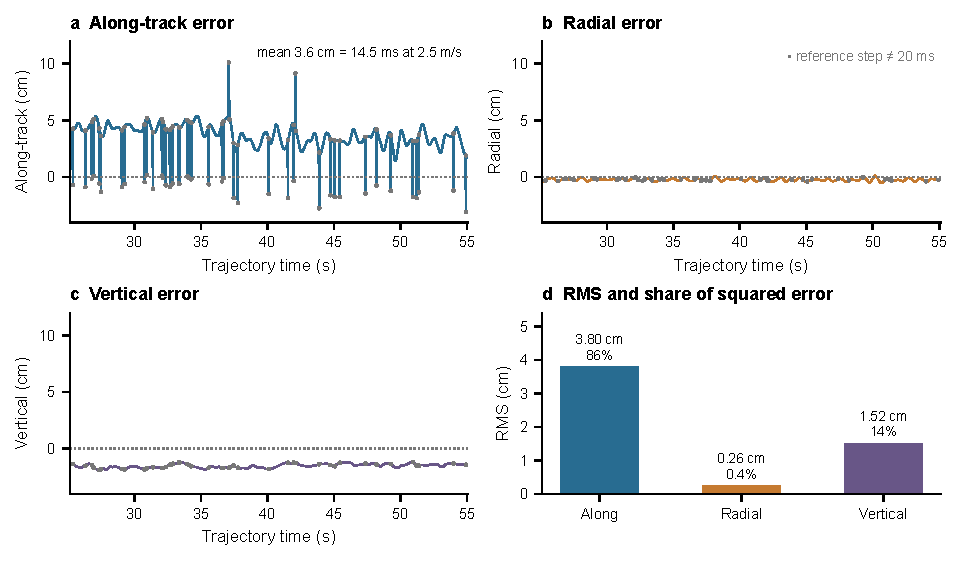
\includegraphics[width=\linewidth]{figures/component_errors.pdf}
\caption{Steady-window error in the reference's moving frame. (a) Along-track, (b) radial and (c) vertical components, on common axes. Grey dots mark samples whose paired reference advanced by 0 or 40 ms. (d) RMS of each component and its share of the mean squared three-dimensional error; the shares sum to 100\%.}
\label{fig:components}
\end{figure}

The vertical component is a steady offset of $-1.51$ cm, which is 13.6\% of the squared error. The commanded thrust explains it exactly (Figure~\ref{fig:commands}a). In the steady window the controller commands $10.10\pm0.04$ N (mean $\pm$ s.d.), while the circle's feedforward for the modelled 1 kg vehicle is $m\|ge_3+a_d\|=9.89$ N. The simulated vehicle therefore needs 0.21 N more than the model supplies. A proportional-only position loop provides it at equilibrium through $k_x|e_z|=14\times0.0151=0.21$ N, which matches the thrust surplus to within 1\%.

\begin{figure}[!htbp]
\centering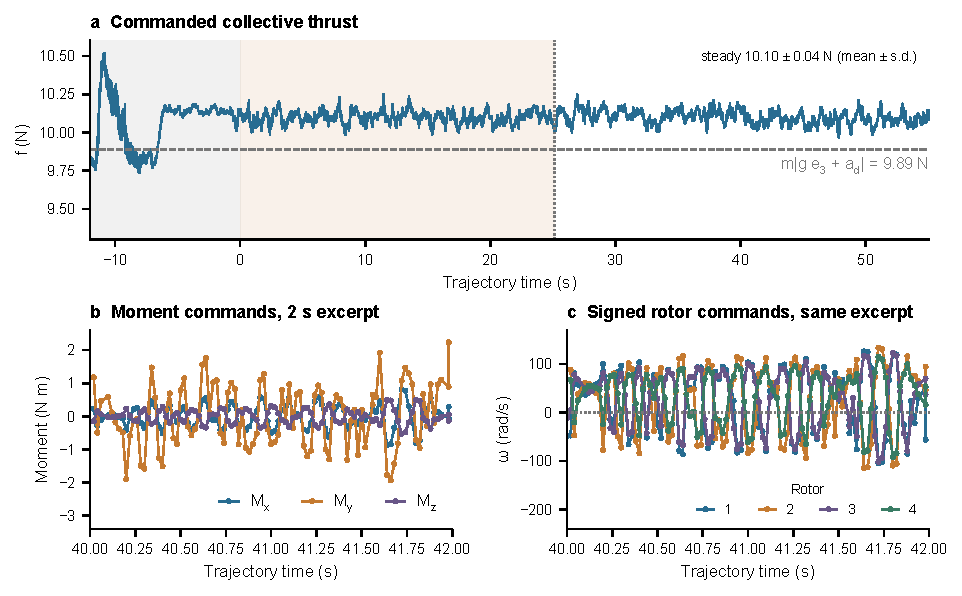
\includegraphics[width=\linewidth]{figures/rotor_commands.pdf}
\caption{Controller output reconstructed through the simulator allocation of Equation~\eqref{eq:fsim}. (a) Collective thrust over the complete flight, from the first published command; the dashed line is the circle feedforward for $m=1$ kg. (b) Body-moment commands and (c) the four signed rotor-speed commands in a 2 s steady excerpt, one marker per logged state sample.}
\label{fig:commands}
\end{figure}

Figure~\ref{fig:commands}b,c shows how the allocation divides the work. Thrust stays smooth, and the high-bandwidth attitude loop acts through the moments, with standard deviations of 0.31, 0.87 and 0.18 N\,m about $x$, $y$ and $z$. Because the moment terms are large compared with the hover share of each rotor, 29\% of the steady rotor commands are negative. The signed allocation passes them to the simulator's reversible rotors, and the reconstructed thrust confirms that the collective channel is unaffected.

\subsection{Start sequence}
Figure~\ref{fig:takeoff} shows the start sequence. The vehicle follows the transfer, hover and rate ramp with a position error of at most 3.4 cm, peaks at 1.988 m with no overshoot of the 2 m target, and turns its heading the short way through $166^\circ$. The angular-rate magnitude peaks at $66^\circ$\,s$^{-1}$ during the transfer, compared with about $400^\circ$\,s$^{-1}$ in the earlier direct start. The position error stays at or below 8.5 cm through the first two periods.

\begin{figure}[!htbp]
\centering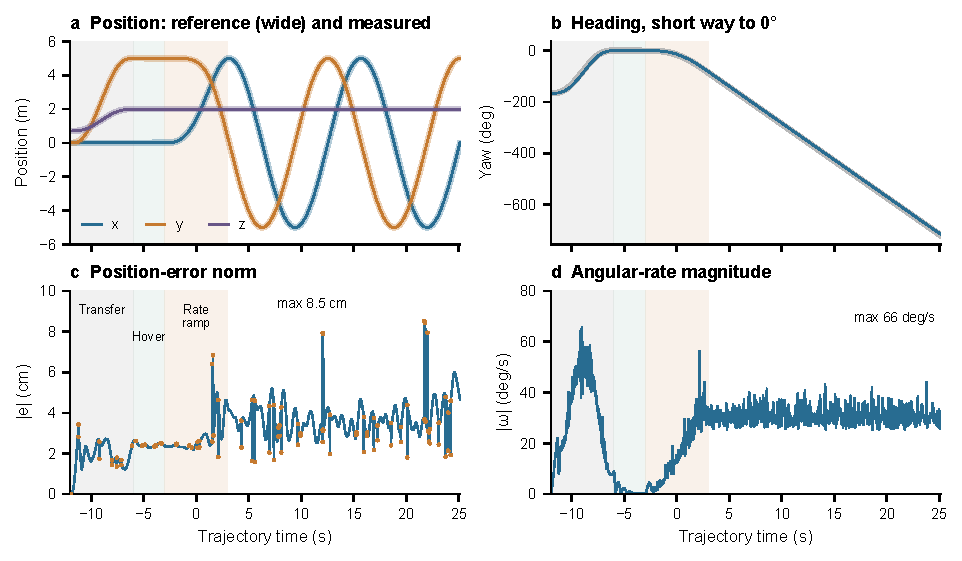
\includegraphics[width=\linewidth]{figures/takeoff_transition.pdf}
\caption{Start sequence and first two periods ($t<8\pi$ s). (a) Position components: reference (wide, light) and measured (thin). (b) Unwrapped heading, reference and measured. (c) Position-error norm; orange dots mark samples whose reference advanced by 0 or 40 ms. (d) Magnitude of the measured angular velocity. Shading marks the 6 s minimum-jerk transfer, the 3 s hover and the 6 s rate ramp centred on $t=0$.}
\label{fig:takeoff}
\end{figure}

\subsection{Gain selection}
State feedback at 50 Hz supports stiff gains. Gains were tuned on 50 s circle runs with the same steady window (Figure~\ref{fig:gains}). The first stiff set, $(k_x,k_v,k_R,k_\Omega)=(14,6,12,2.2)$, already reached 5.1 cm. Raising the attitude gains from $(k_R,k_\Omega)=(12,2.2)$ to $(20,3)$ then lowered it to 3.7 cm and the radial RMS error from 7 mm to 3 mm, reproduced on a repeat run. Pushing the position loop to $(20,8)$ with the softer attitude gains made the vehicle unstable. This marks the boundary: the attitude loop must stay fast relative to the position loop. The final flight, which also includes the start sequence, confirms the selected gains at 4.1 cm.

\begin{figure}[!htbp]
\centering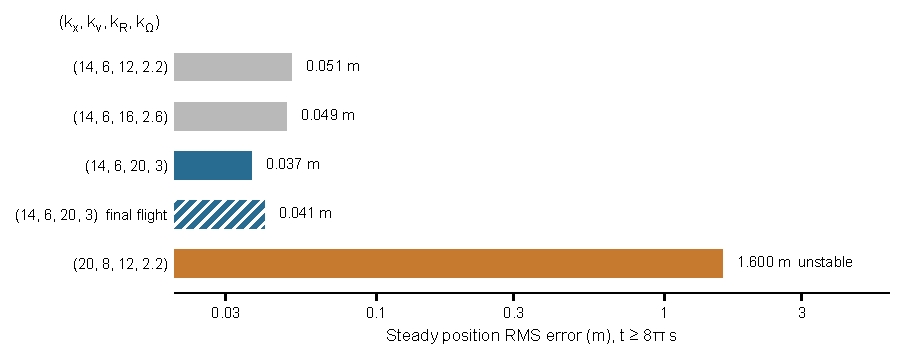
\includegraphics[width=.95\linewidth]{figures/gain_comparison.pdf}
\caption{Gain selection. Steady position RMS error ($t\geq8\pi$ s, log scale) for each gain set, one 50 s circle run per set, from the tuning record kept with the run. The hatched bar is the final flight reported in Figures~\ref{fig:tracking}--\ref{fig:takeoff}.}
\label{fig:gains}
\end{figure}

\subsection{Simulator and RViz recordings}
Unity and RViz were recorded at the same time, each for 69.3 s at 30 fps and real-time speed: \texttt{report/video/unity\_gpu\_sim.mp4} and \texttt{report/video/rviz\_gpu.mp4}. In RViz the cyan measured path keeps the last lap. Once the start transient has scrolled out, the path sits entirely under the yellow desired circle (Figure~\ref{fig:views}b), which is the 2.4 mm radial error made visible at room scale.

\begin{figure}[!htbp]
\centering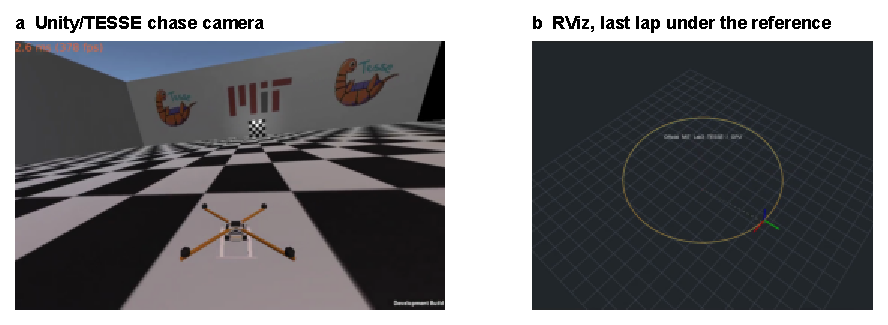
\includegraphics[width=\linewidth]{figures/simulator_views.pdf}
\caption{Unmodified frames from the synchronised recordings. (a) Unity/TESSE chase camera at 40 s; the overlay reports the frame time. (b) RViz 3D view at 64 s, cropped to the viewport: desired circle (yellow), measured path (cyan, hidden under the circle), desired frame and vehicle frame.}
\label{fig:views}
\end{figure}

\section{Discussion}
The allocation proof identifies a structural requirement for tracking position and yaw independently. The original layout spans all four wrench directions. In the modified layout the yaw moment is tied to the roll moment, so no feedback gain can recover the missing direction. The simulator matrix of Equation~\eqref{eq:fsim} shows the same lesson in practice: rotor numbering and yaw signs must be matched to the plant, not copied from the exercise.

The flight shows what the geometric controller achieves once the plant delivers state at a steady rate. The geometry of the circle is reproduced to millimetres, and the residual error has two identifiable sources. The along-track offset comes from pairing each state with the most recent reference message. Stamping the reference by state time, or logging the reference evaluated at the state's timestamp, would remove most of the 86\% share without changing the controller. The vertical offset is the equilibrium of a proportional loop against a 0.21 N model mismatch. Raising $m$ to the simulator's effective mass, or adding integral action on $e_z$, removes it.

The start sequence matters as much as the gains. Joining the circle with continuous position, velocity and acceleration lets the stiff attitude gains act on small errors from the first sample, so the vehicle enters the official reference at full accuracy without any transient exclusion beyond the standard two periods.

The drag term has a well-defined role: it cancels a specified force model, and the independent numerical runs confirm a 75.6\% error reduction when the plant includes that model. The same structure applies to TESSE once its effective drag is identified, alongside the 0.21 N thrust correction above.

\section{Conclusions}
The lab connects quaternion conversion and rotor allocation to a working ROS geometric controller. The rank proof shows that reversing two rotors removes independent yaw authority, and the drag model yields an exact force correction. In the TESSE simulator, the controller holds the 5 m circle to 2.4 mm radial RMS error and 4.1 cm three-dimensional RMS error. A smooth start sequence brings the vehicle from its spawn pose onto the circle without overshoot. The remaining error splits into a 14.5 ms reference-timing offset and a 1.5 cm height offset matching the measured 0.21 N thrust surplus, so both can be removed with the targeted changes identified above.

\bibliographystyle{unsrtnat}
\bibliography{references}
\end{document}
